% Options for packages loaded elsewhere
\PassOptionsToPackage{unicode}{hyperref}
\PassOptionsToPackage{hyphens}{url}
\PassOptionsToPackage{dvipsnames,svgnames*,x11names*}{xcolor}
%
\documentclass[
]{article}
\usepackage{lmodern}
\usepackage{amssymb,amsmath}
\usepackage{ifxetex,ifluatex}
\ifnum 0\ifxetex 1\fi\ifluatex 1\fi=0 % if pdftex
  \usepackage[T1]{fontenc}
  \usepackage[utf8]{inputenc}
  \usepackage{textcomp} % provide euro and other symbols
\else % if luatex or xetex
  \usepackage{unicode-math}
  \defaultfontfeatures{Scale=MatchLowercase}
  \defaultfontfeatures[\rmfamily]{Ligatures=TeX,Scale=1}
\fi
% Use upquote if available, for straight quotes in verbatim environments
\IfFileExists{upquote.sty}{\usepackage{upquote}}{}
\IfFileExists{microtype.sty}{% use microtype if available
  \usepackage[]{microtype}
  \UseMicrotypeSet[protrusion]{basicmath} % disable protrusion for tt fonts
}{}
\makeatletter
\@ifundefined{KOMAClassName}{% if non-KOMA class
  \IfFileExists{parskip.sty}{%
    \usepackage{parskip}
  }{% else
    \setlength{\parindent}{0pt}
    \setlength{\parskip}{6pt plus 2pt minus 1pt}}
}{% if KOMA class
  \KOMAoptions{parskip=half}}
\makeatother
\usepackage{xcolor}
\IfFileExists{xurl.sty}{\usepackage{xurl}}{} % add URL line breaks if available
\IfFileExists{bookmark.sty}{\usepackage{bookmark}}{\usepackage{hyperref}}
\hypersetup{
  colorlinks=true,
  linkcolor=blue,
  filecolor=Maroon,
  citecolor=Blue,
  urlcolor=Blue,
  pdfcreator={LaTeX via pandoc}}
\urlstyle{same} % disable monospaced font for URLs
\usepackage{graphicx}
\makeatletter
\def\maxwidth{\ifdim\Gin@nat@width>\linewidth\linewidth\else\Gin@nat@width\fi}
\def\maxheight{\ifdim\Gin@nat@height>\textheight\textheight\else\Gin@nat@height\fi}
\makeatother
% Scale images if necessary, so that they will not overflow the page
% margins by default, and it is still possible to overwrite the defaults
% using explicit options in \includegraphics[width, height, ...]{}
\setkeys{Gin}{width=\maxwidth,height=\maxheight,keepaspectratio}
% Set default figure placement to htbp
\makeatletter
\def\fps@figure{htbp}
\makeatother
\setlength{\emergencystretch}{3em} % prevent overfull lines
\providecommand{\tightlist}{%
  \setlength{\itemsep}{0pt}\setlength{\parskip}{0pt}}
\setcounter{secnumdepth}{5}

%% pandoc-secnos: required package
\usepackage{cleveref}

\author{}
\date{}

\begin{document}

\newcommand{\Ber}{\operatorname{Ber}}
\newcommand{\E}{\operatorname{E}}
\newcommand{\V}{\operatorname{Var}}
\newcommand{\diag}{\operatorname{diag}}

\newcommand{\bi}{\mathbf{i}}
\newcommand{\bj}{\mathbf{j}}
\newcommand{\bt}{\mathbf{t}}

\newcommand{\bw}{{\boldsymbol{w}}}
\newcommand{\bu}{{\boldsymbol{u}}}
\newcommand{\bv}{{\boldsymbol{v}}}
\newcommand{\bx}{{\boldsymbol{x}}}
\newcommand{\by}{{\boldsymbol{y}}}
\newcommand{\bb}{{\boldsymbol{b}}}
\newcommand{\bz}{{\boldsymbol{z}}}
\newcommand{\bX}{{\boldsymbol{X}}}
\newcommand{\bY}{{\boldsymbol{Y}}}
\newcommand{\bZ}{{\boldsymbol{Z}}}

\hypertarget{gradient-descent}{%
\section{Gradient Descent}\label{gradient-descent}}

\hypertarget{motivation}{%
\subsection{Motivation}\label{motivation}}

In Linear Regression, we studied how to minimize the error function
\[ E = \sum_{j=1}^{N} (y_j-\sum_{s=1}^{k+1} x_{js}m_{s})^2 \] and
obtained an exact solution. In other cases we will encounter later, such
an exact solution is not feasible and we will have to use a method to
approximate an exact solution. One of the most common methods for this
purpose is \emph{gradient descent}.

\hypertarget{basic-algorithm}{%
\subsection{Basic Algorithm}\label{basic-algorithm}}

Consider a function \(E: \mathbb R^n \rightarrow \mathbb R\),
\({\boldsymbol{w}}=(w_1, w_2, \dots , w_n) \rightarrow E({\boldsymbol{w}})\).
The \emph{gradient} \(\nabla E\) of \(E\) is defined by
\[  \nabla E := \left ( \frac {\partial E}{\partial w_1}, \frac {\partial E}{\partial w_2}, \dots , \frac {\partial E}{\partial w_n} \right ). \]

\textbf{Proposition }: \emph{Assume that \(E({\boldsymbol{w}})\) is
differentiable in a neighborhood of \({\boldsymbol{w}}\). Then the
function \(E({\boldsymbol{w}})\) decreases fastest in the direction of
\(-\nabla E ({\boldsymbol{w}})\).}

\textbf{Proof:} For a unit vector \({\boldsymbol{u}}\), the directional
derivative \(D_{\boldsymbol{u}}E\) is given by
\[ D_{\boldsymbol{u}}E= \nabla E \cdot {\boldsymbol{u}}= | \nabla E | |{\boldsymbol{u}}| \cos \theta = | \nabla E | \cos \theta ,\]
where \(\theta\) is the angle between \(\nabla E\) and
\({\boldsymbol{u}}\). The minimum value of \(D_{\boldsymbol{u}}E\)
occurs when \(\cos \theta\) is \(-1\). ~ ~ \(\square\)

Set
\[ {\boldsymbol{w}}_{k+1}={\boldsymbol{w}}_k - \eta \nabla E({\boldsymbol{w}}_k) \]
where \(\eta >0\) is the step size or \emph{learning rate}. Then
\[ E({\boldsymbol{w}}_{k+1}) \le E({\boldsymbol{w}}_{k}).\] Under some
moderate conditions,
\[ E({\boldsymbol{w}}_k) \rightarrow \text{local minimum} \qquad \text{ as }\ k \rightarrow \infty .\]In
particular, this is true when \(E\) is convex or when \(\nabla E\) is
Lipschitz continuous.

\hypertarget{example}{%
\subsubsection{Example}\label{example}}

Consider \(E({\boldsymbol{w}})=E(w_1,w_2)= w_1^4+w_2^4-16w_1w_2\). Then
\(\nabla E({\boldsymbol{w}})= [ 4w_1^3-16w_2, 4w_2^3-16w_1]\). Choose
\({\boldsymbol{w}}_0=(1,1)\) and \(\eta =0.01\). Then
\[ {\boldsymbol{w}}_{30}=(1.99995558586289, 1.99995558586289)\] and we
get \[ E({\boldsymbol{w}}_{30})= -31.9999999368777. \]

We see that \({\boldsymbol{w}}_k \rightarrow (2,2)\) and \(E(2,2)=-32\).
Indeed, using multi-variable calculus, one can verify that when
\({\boldsymbol{w}}=(2,2)\), a local minimum of \(E({\boldsymbol{w}})\)
is \(-32\).

\textbf{Exercise}: Using multi-variable calculus, find all the local
minima of \(E({\boldsymbol{w}})\).

\begin{figure}
\hypertarget{fig:des}{%
\centering
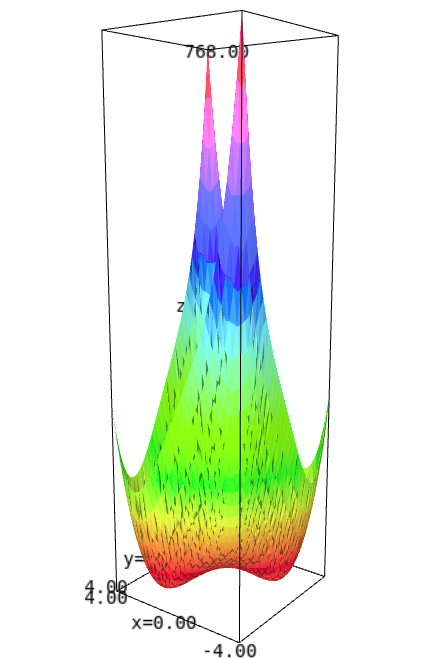
\includegraphics[width=0.3\textwidth,height=\textheight]{descent.png}
\caption{Graph of \(E({\boldsymbol{w}})\)}\label{fig:des}
}
\end{figure}

\begin{figure}
\hypertarget{fig:tab}{%
\centering
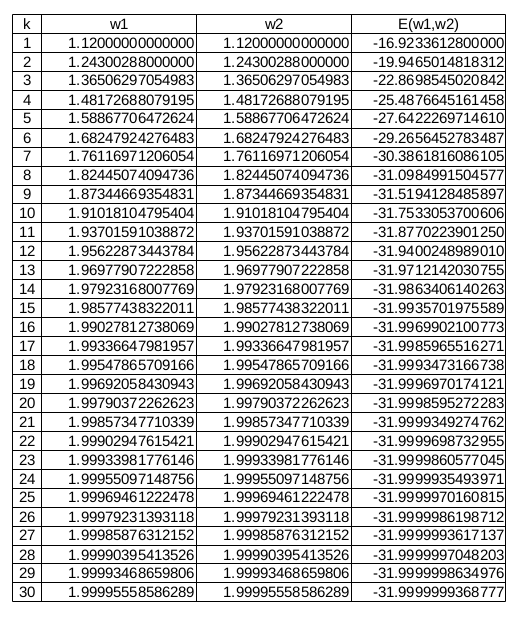
\includegraphics[width=0.5\textwidth,height=\textheight]{table.png}
\caption{Values of \(E({\boldsymbol{w}}_k)\)}\label{fig:tab}
}
\end{figure}

\hypertarget{example-linear-regression-revisited}{%
\subsubsection{Example: Linear Regression
revisited}\label{example-linear-regression-revisited}}

We will apply gradient descent to linear regression in the lab session.

\textbf{Exercise}: Define
\(\sigma(x) = \dfrac {e^x}{e^x+1}= \dfrac 1 {1+e^{-x}}\). In Logistic
Regression we will minimize the following error function
\[ E ({\boldsymbol{w}}) = - \sum_{n=1}^N \{ t_n \ln y_n + (1-t_n) \ln (1-y_n)\},  \]
where we write \({\boldsymbol{w}}=(w_1, w_2, \dots , w_{k+1})\) and
\(y_n=\sigma(w_1 x_{n1}+ w_2 x_{n2} + \cdots + w_k x_{nk}+w_{k+1} )\).
Compute the gradient \(\nabla E({\boldsymbol{w}})\).

\hypertarget{newtons-method}{%
\subsection{Newton's Method}\label{newtons-method}}

Let us first consider the single-variable case.

\begin{itemize}
\item
  Let \(f: \mathbb R \longrightarrow \mathbb R\) be a single-variable
  (convex, differentiable) function.
\item
  To find a local minimum \(\Longleftrightarrow\) \qquad To find \(x^*\)
  such that \(f'(x^*)=0\)\\
  Make a guess \(x_0\) for \(x^*\) and set \(x=x_0+h\).
\item
  Using the Taylor expansion, we have
  \begin{align*} f(x) &=f(x_0+h) \approx f(x_0) + f'(x_0) h+ \tfrac 1 2 f''(x_0) h^2 \\ f'(x) = \frac{df}{dh}\frac {dh}{dx} & \approx \frac d {dh} \left ( f(x_0) + f'(x_0) h+ \tfrac 1 2 f''(x_0) h^2 \right ) \\
  &= f'(x_0) + f''(x_0)h \end{align*} If \(0 = f'(x_0) + f''(x_0)h\), we
  obtain \[ h = - f'(x_0)/f''(x_0). \]
\item
  We have shown that \[ x_1=x_0- f'(x_0)/f''(x_0) \] is an approximation
  of \(x^*\).
\item
  Repeat the process to obtain
  \[ \boxed{x_{k+1}=x_k- f'(x_k)/f''(x_k)},  \] and
  \(x_k \rightarrow x^*\) as \(k \rightarrow \infty\).
\end{itemize}

Now we consider the multi-variable case.

\begin{itemize}
\item
  Let \(E({\boldsymbol{w}})\) be a multi-variable function. The
  \emph{Hessian matrix} of \(E\) is defined by
  \[ \mathbf H E= \begin{bmatrix} \tfrac {\partial^2 E}{\partial w_1^2} &  \tfrac {\partial^2 E}{\partial w_1 \partial w_2} & \cdots &  \tfrac {\partial^2 E}{\partial w_1 \partial w_n} \\ \tfrac {\partial^2 E}{\partial w_2 \partial w_1} & \tfrac {\partial^2 E}{\partial w_2^2} & \cdots & \tfrac {\partial^2 E}{\partial w_2 \partial w_n} \\ \vdots & \vdots & \ddots & \vdots \\ \tfrac {\partial^2 E}{\partial w_n \partial w_1} & \tfrac {\partial^2 E}{\partial w_n \partial w_2} & \cdots & \tfrac {\partial^2 E}{\partial w_n^2}  \end{bmatrix}. \]
  That is,
  \(\mathbf H E= [ \tfrac {\partial^2 E}{\partial w_i \partial w_j}]\).
\item
  Generalizing the single-variable case, we obtain\\
  \[ \boxed{ {\boldsymbol{w}}_{k+1}= {\boldsymbol{w}}_k - \mathbf H E ({\boldsymbol{w}}_{k})^{-1} \nabla E({\boldsymbol{w}}_k)} . \]
\item
  Using a step size \(\eta\), the formula may be modified to be
  \[  \boxed{ {\boldsymbol{w}}_{k+1}= {\boldsymbol{w}}_k - \eta \mathbf H E ({\boldsymbol{w}}_{k})^{-1} \nabla E({\boldsymbol{w}}_k)} . \]
\item
  Newton's method is much faster than Gradient Descent. However, it may
  be expensive to compute the inverse of the Hessian matrix.
\end{itemize}

\hypertarget{example-1}{%
\subsubsection{Example}\label{example-1}}

\begin{itemize}
\tightlist
\item
  Consider \(E({\boldsymbol{w}})=E(w_1,w_2)= w_1^4+w_2^4-16w_1w_2\).
  Then
  \(\nabla E({\boldsymbol{w}})= [ 4w_1^3-16w_2, 4w_2^3-16w_1]^\top\).
\end{itemize}

\begin{align*} \mathbf H E({\boldsymbol{w}}) &= \begin{bmatrix} 12 w_1^2 & -16 \\ -16 & 12 w_2^2 \end{bmatrix} \\ \\ \mathbf H E({\boldsymbol{w}})^{-1} &= \frac 1 {9w_1^2 w_2^2 -16} \begin{bmatrix} \tfrac 3 4 w_2^2 & 1 \\ 1& \frac 3 4 w_1^2  \end{bmatrix} \\  \\
\mathbf H E^{-1} \nabla E & = \frac 1 {9w_1^2 w_2^2 -16} \begin{bmatrix} 3 w_1^3 w_2^2 -8 w_2^3 -16w_1 \\ 3 w_1^2 w_2^3 -8 w_1^3  -16w_2  \end{bmatrix} \end{align*}

\begin{itemize}
\tightlist
\item
  Choose \({\boldsymbol{w}}_0=(1.2,1.2)\) and \(\eta =1\). Then
  \({\boldsymbol{w}}_{9}=(2.00000004189571, 2.00000004189571)\),
  \(E({\boldsymbol{w}}_{9})= -31.9999999999999\).
\end{itemize}

\begin{figure}
\hypertarget{fig:tab}{%
\centering
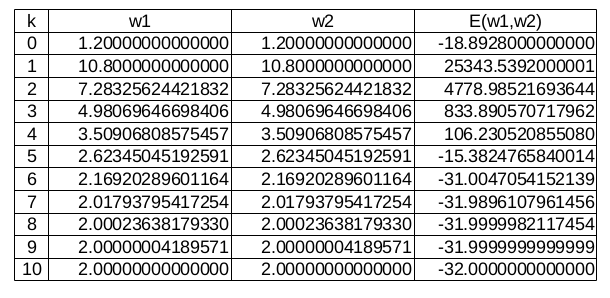
\includegraphics[width=0.5\textwidth,height=\textheight]{table-1.png}
\caption{Values of \(E({\boldsymbol{w}}_k)\)}\label{fig:tab}
}
\end{figure}

\hypertarget{stochastic-gradient-descent-sgd}{%
\subsubsection{Stochastic Gradient Descent
(SGD)}\label{stochastic-gradient-descent-sgd}}

Typically in Machine Learning, the function \(E({\boldsymbol{w}})\) is
given by a sum of the form
\[ E({\boldsymbol{w}}) = \frac 1 N \sum_{n=1}^N E_n({\boldsymbol{w}}), \]
where \(N\) is the number of elements in the training set. When \(N\) is
large, computation of the gradient \(\nabla E\) may be expensive.

The SGD selects a sample from the training set in each iteration step
instead of using the whole batch of the training set, and use
\[ \frac 1 M \sum_{i=1}^M \nabla E_{n_i}({\boldsymbol{w}}) ,\] where
\(M\) is the size of the sample and
\(\{ n_1, n_2 , \dots , n_M \} \subset \{ 1,2, \dots , N \}\). The SGD
is commonly used in many Machine Learning algorithms.

\end{document}
